% GreyKT-v3 detailed architecture (English). Compiles with plain pdflatex.
% Arrow routing is fully orthogonal; the two long "response feed" dotted lines
% from the earlier draft were removed because r_t and y_tau already appear in
% the box formulas -- the arrows carried no information the boxes did not.
\documentclass[tikz,border=8pt]{standalone}
\usepackage{tikz}
\usetikzlibrary{positioning,fit,shapes.geometric,backgrounds,calc,arrows.meta}
\usepackage{amsmath}
\begin{document}
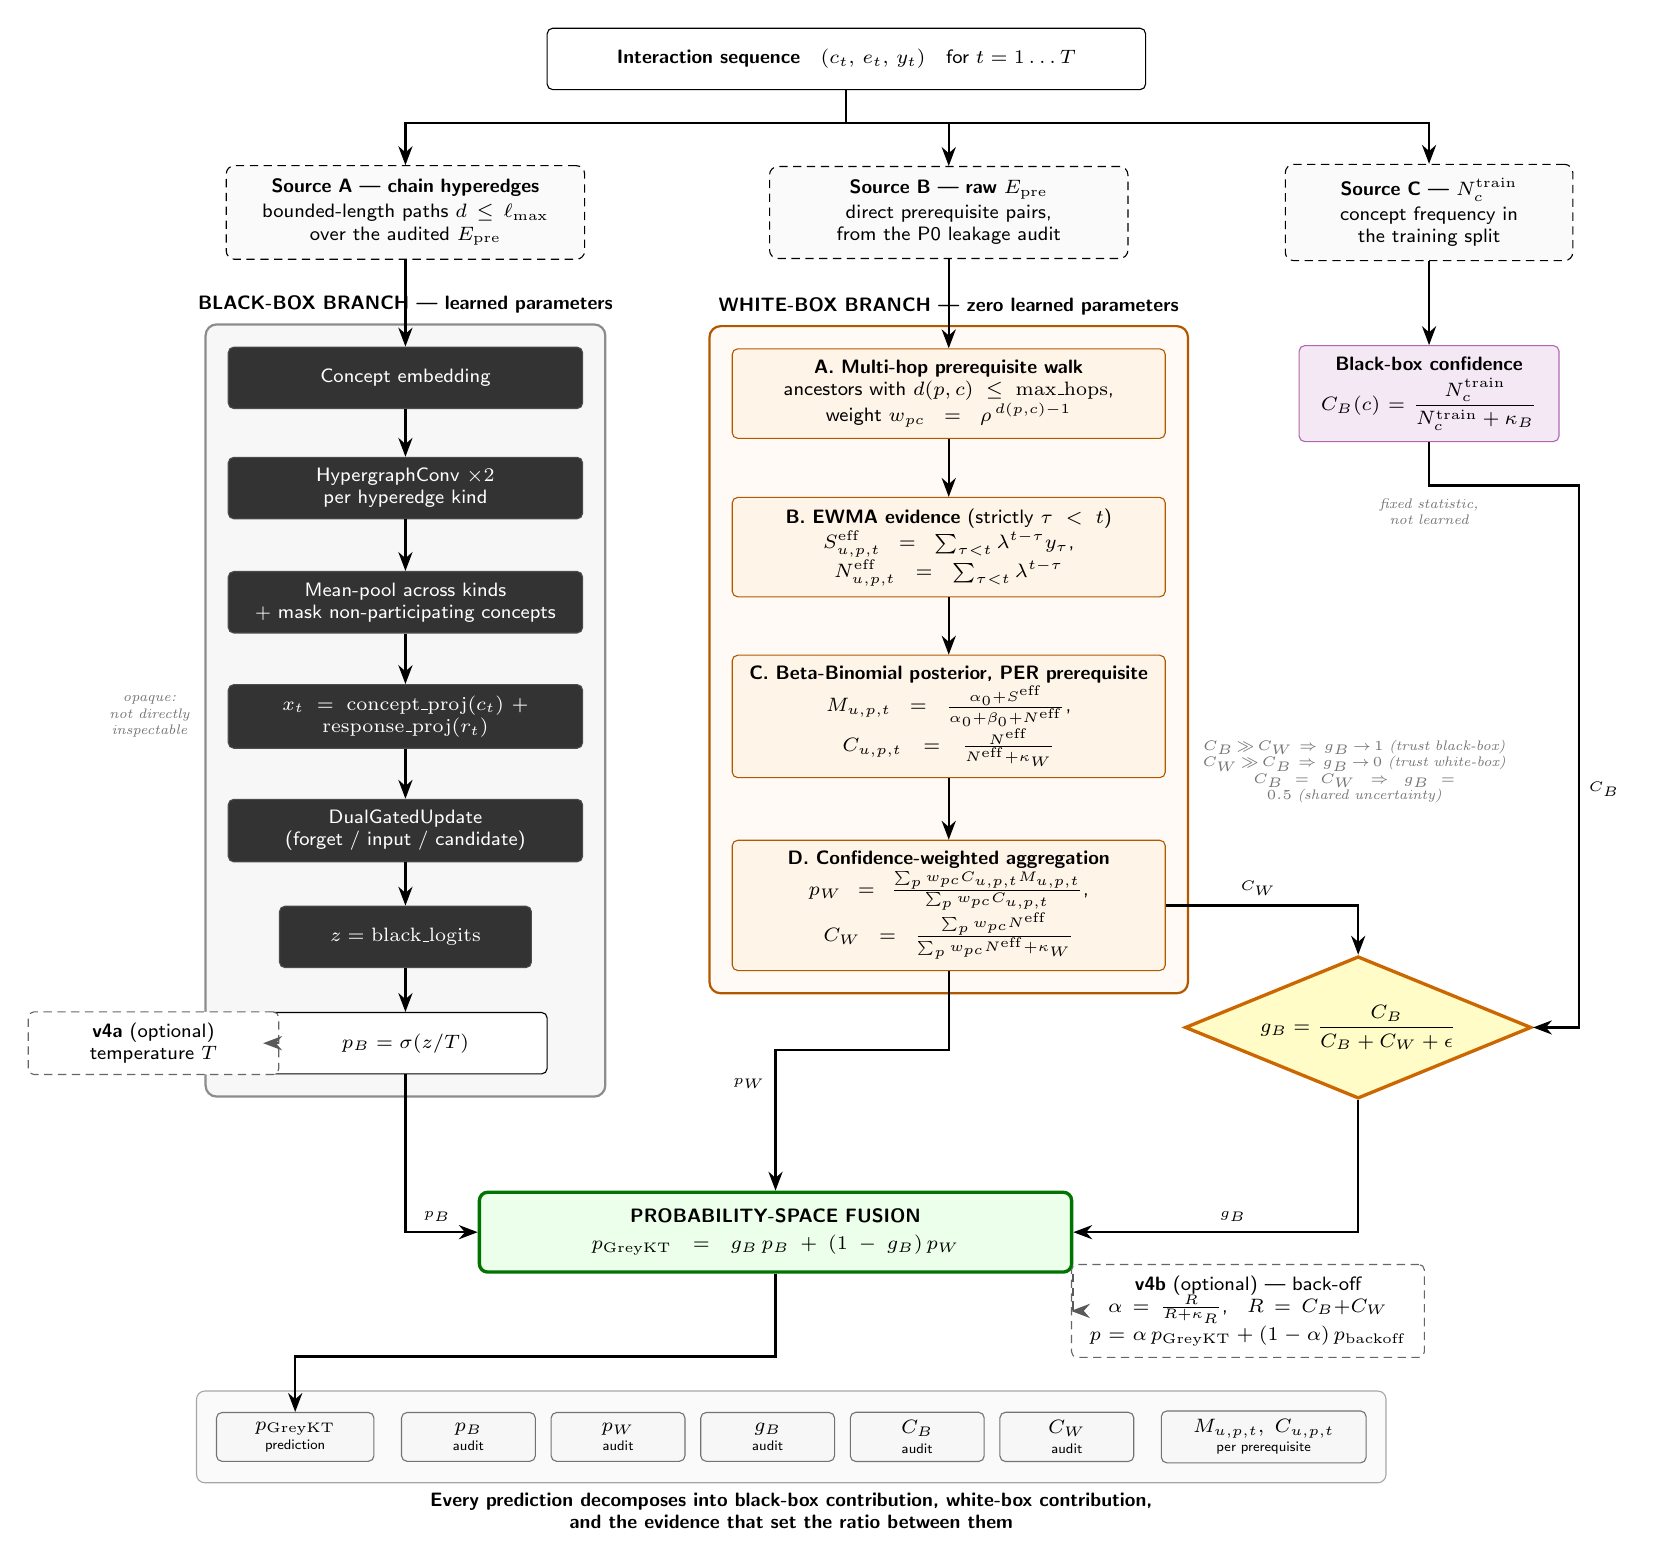
\begin{tikzpicture}[
  font=\scriptsize\sffamily,
  >={Stealth[length=2.4mm,width=1.8mm]},
  box/.style={draw, rounded corners=2pt, align=center, inner sep=4pt,
              minimum height=0.78cm, fill=white},
  dark/.style={draw=black!70, rounded corners=2pt, align=center, inner sep=4pt,
               minimum height=0.78cm, fill=black!80, text=white},
  amber/.style={draw=orange!70!black, rounded corners=2pt, align=center, inner sep=4pt,
                minimum height=0.78cm, fill=orange!9},
  viol/.style={draw=violet!60, rounded corners=2pt, align=center, inner sep=4pt,
               minimum height=0.78cm, fill=violet!9},
  art/.style={draw, densely dashed, rounded corners=3pt, align=center, inner sep=5pt, fill=black!2},
  gatebox/.style={draw=orange!80!black, very thick, diamond, aspect=2.4, align=center,
                  inner sep=2pt, fill=yellow!22},
  fuse/.style={draw=green!45!black, very thick, rounded corners=3pt, align=center,
               inner sep=6pt, fill=green!8},
  outbox/.style={draw=black!55, rounded corners=2pt, align=center, inner sep=3pt,
                 minimum height=0.62cm, fill=black!3},
  opt/.style={draw=black!60, densely dashed, rounded corners=2pt, align=center,
              inner sep=4pt, fill=white},
  hdr/.style={font=\scriptsize\bfseries\sffamily},
  tag/.style={font=\tiny\itshape, text=black!55},
  flow/.style={->, thick},
  aux/.style={->, thick, densely dashed, black!65},
]

% ============================== INPUT ==============================
\node[box, minimum width=7.6cm] (seq) at (8.3,0)
  {\textbf{Interaction sequence}\quad $(c_t,\,e_t,\,y_t)$\quad for $t=1\ldots T$};

% ============================== SOURCES ==============================
\node[art, text width=4.2cm] (artA) at (2.7,-1.95)
  {\textbf{Source A --- chain hyperedges}\\[1pt]
   bounded-length paths $d\le\ell_{\max}$\\ over the audited $E_{\mathrm{pre}}$};
\node[art, text width=4.2cm] (artB) at (9.6,-1.95)
  {\textbf{Source B --- raw $E_{\mathrm{pre}}$}\\[1pt]
   direct prerequisite pairs,\\ from the P0 leakage audit};
\node[art, text width=3.3cm] (artC) at (15.7,-1.95)
  {\textbf{Source C --- $N_c^{\mathrm{train}}$}\\[1pt]
   concept frequency in\\ the training split};

\draw[flow] (seq.south) -- ++(0,-0.42) -| (artA.north);
\draw[flow] (seq.south) -- ++(0,-0.42) -| (artB.north);
\draw[flow] (seq.south) -- ++(0,-0.42) -| (artC.north);

% ============================== BLACK-BOX BRANCH ==============================
\node[dark, minimum width=4.5cm] (b1) at (2.7,-4.05) {Concept embedding};
\node[dark, minimum width=4.5cm, text width=4.2cm] (b2) at (2.7,-5.45)
  {HypergraphConv $\times 2$\\ per hyperedge kind};
\node[dark, minimum width=4.5cm, text width=4.2cm] (b3) at (2.7,-6.9)
  {Mean-pool across kinds\\ + mask non-participating concepts};
\node[dark, minimum width=4.5cm, text width=4.2cm] (b4) at (2.7,-8.35)
  {$x_t=\mathrm{concept\_proj}(c_t)+\mathrm{response\_proj}(r_t)$};
\node[dark, minimum width=4.5cm, text width=4.2cm] (b5) at (2.7,-9.8)
  {DualGatedUpdate\\ (forget / input / candidate)};
\node[dark, minimum width=3.2cm] (b6) at (2.7,-11.15) {$z=\mathrm{black\_logits}$};
\node[box, minimum width=3.6cm] (b7) at (2.7,-12.5) {$p_B=\sigma(z/T)$};

\foreach \a/\b in {artA/b1, b1/b2, b2/b3, b3/b4, b4/b5, b5/b6, b6/b7}
  \draw[flow] (\a) -- (\b);

\node[tag, text width=1.9cm, align=center] at (-0.55,-8.35)
  {opaque:\\ not directly\\ inspectable};

\begin{pgfonlayer}{background}
\node[draw=black!45, thick, rounded corners=4pt, fill=black!3, inner sep=8pt,
      fit=(b1)(b2)(b3)(b4)(b5)(b6)(b7),
      label={[hdr]above:BLACK-BOX BRANCH --- learned parameters}] {};
\end{pgfonlayer}

% ============================== WHITE-BOX BRANCH ==============================
\node[amber, minimum width=5.5cm, text width=5.2cm] (w1) at (9.6,-4.25)
  {\textbf{A. Multi-hop prerequisite walk}\\
   ancestors with $d(p,c)\le \mathrm{max\_hops}$,\\
   weight $w_{pc}=\rho^{\,d(p,c)-1}$};
\node[amber, minimum width=5.5cm, text width=5.2cm] (w2) at (9.6,-6.2)
  {\textbf{B. EWMA evidence} (strictly $\tau<t$)\\
   $S^{\mathrm{eff}}_{u,p,t}=\sum_{\tau<t}\lambda^{t-\tau}y_\tau$,\quad
   $N^{\mathrm{eff}}_{u,p,t}=\sum_{\tau<t}\lambda^{t-\tau}$};
\node[amber, minimum width=5.5cm, text width=5.2cm] (w3) at (9.6,-8.35)
  {\textbf{C. Beta-Binomial posterior, PER prerequisite}\\
   $M_{u,p,t}=\frac{\alpha_0+S^{\mathrm{eff}}}{\alpha_0+\beta_0+N^{\mathrm{eff}}}$,\quad
   $C_{u,p,t}=\frac{N^{\mathrm{eff}}}{N^{\mathrm{eff}}+\kappa_W}$};
\node[amber, minimum width=5.5cm, text width=5.2cm] (w4) at (9.6,-10.75)
  {\textbf{D. Confidence-weighted aggregation}\\
   $p_W=\frac{\sum_p w_{pc}C_{u,p,t}M_{u,p,t}}{\sum_p w_{pc}C_{u,p,t}}$,\quad
   $C_W=\frac{\sum_p w_{pc}N^{\mathrm{eff}}}{\sum_p w_{pc}N^{\mathrm{eff}}+\kappa_W}$};

\foreach \a/\b in {artB/w1, w1/w2, w2/w3, w3/w4}
  \draw[flow] (\a) -- (\b);

\begin{pgfonlayer}{background}
\node[draw=orange!70!black, thick, rounded corners=4pt, fill=orange!4, inner sep=8pt,
      fit=(w1)(w2)(w3)(w4),
      label={[hdr]above:WHITE-BOX BRANCH --- zero learned parameters}] {};
\end{pgfonlayer}

% ============================== BLACK-BOX CONFIDENCE ==============================
\node[viol, minimum width=3.3cm, text width=3.0cm] (cb) at (15.7,-4.25)
  {\textbf{Black-box confidence}\\[2pt]
   $C_B(c)=\dfrac{N_c^{\mathrm{train}}}{N_c^{\mathrm{train}}+\kappa_B}$};
\draw[flow] (artC) -- (cb);
\node[tag, text width=3.1cm, align=center] at (15.7,-5.75)
  {fixed statistic,\\ not learned};

% ============================== GATE ==============================
\node[gatebox, minimum width=4.4cm] (g) at (14.8,-12.3)
  {$g_B=\dfrac{C_B}{C_B+C_W+\epsilon}$};

% C_B travels straight down the right margin, clear of every box.
\draw[flow] (cb.south) -- ++(0,-0.55) -- ++(1.9,0) |- node[right, font=\tiny, pos=0.28] {$C_B$} (g.east);
% C_W leaves the white-box branch on its right edge.
\draw[flow] (w4.east) -| node[above, font=\tiny, pos=0.24] {$C_W$} (g.north);

\node[tag, text width=3.9cm, align=center] at (14.75,-9.05)
  {$C_B\!\gg\!C_W\Rightarrow g_B\!\to\!1$ (trust black-box)\\
   $C_W\!\gg\!C_B\Rightarrow g_B\!\to\!0$ (trust white-box)\\
   $C_B\!=\!C_W\Rightarrow g_B\!=\!0.5$ (shared uncertainty)};

% ============================== FUSION ==============================
\node[fuse, minimum width=7.4cm, text width=7.1cm] (f) at (7.4,-14.9)
  {\textbf{PROBABILITY-SPACE FUSION}\\[2pt]
   $p_{\mathrm{GreyKT}}=g_B\,p_B+(1-g_B)\,p_W$};

% p_B: straight down the left margin, then right into the fusion box.
\draw[flow] (b7.south) |- node[above, font=\tiny, pos=0.72] {$p_B$} (f.west);
% p_W: leaves the white-box branch on its left edge, drops, enters from above.
\draw[flow] (w4.south) -- ++(0,-1.0) -| node[left, font=\tiny, pos=0.62] {$p_W$} (f.north);
% g_B: from the gate, down and left into the fusion box.
\draw[flow] (g.south) |- node[above, font=\tiny, pos=0.72] {$g_B$} (f.east);

% ============================== OPTIONAL v4a / v4b ==============================
\node[opt, text width=2.9cm] (v4a) at (-0.5,-12.5)
  {\textbf{v4a} (optional)\\ temperature $T$};
\draw[aux] (v4a.east) -- (b7.west);

\node[opt, text width=4.2cm] (v4b) at (13.4,-15.9)
  {\textbf{v4b} (optional) --- back-off\\
   $\alpha=\frac{R}{R+\kappa_R}$, \; $R=C_B{+}C_W$\\
   $p=\alpha\,p_{\mathrm{GreyKT}}+(1-\alpha)\,p_{\mathrm{backoff}}$};
\draw[aux] (f.south east) |- (v4b.west);

% ============================== AUDIT OUTPUTS ==============================
\node[outbox, minimum width=2.0cm] (o1) at (1.3,-17.5) {$p_{\mathrm{GreyKT}}$\\[-1pt] \tiny prediction};
\node[outbox, minimum width=1.7cm] (o2) at (3.5,-17.5) {$p_B$\\[-1pt] \tiny audit};
\node[outbox, minimum width=1.7cm] (o3) at (5.4,-17.5) {$p_W$\\[-1pt] \tiny audit};
\node[outbox, minimum width=1.7cm] (o4) at (7.3,-17.5) {$g_B$\\[-1pt] \tiny audit};
\node[outbox, minimum width=1.7cm] (o5) at (9.2,-17.5) {$C_B$\\[-1pt] \tiny audit};
\node[outbox, minimum width=1.7cm] (o6) at (11.1,-17.5) {$C_W$\\[-1pt] \tiny audit};
\node[outbox, minimum width=2.6cm] (o7) at (13.6,-17.5)
  {$M_{u,p,t},\;C_{u,p,t}$\\[-1pt] \tiny per prerequisite};

\draw[flow] (f.south) -- ++(0,-1.05) -| (o1.north);

\begin{pgfonlayer}{background}
\node[draw=black!35, rounded corners=3pt, fill=black!2, inner sep=7pt,
      fit=(o1)(o2)(o3)(o4)(o5)(o6)(o7),
      label={[hdr, text width=15cm, align=center]below:Every prediction decomposes into
             black-box contribution, white-box contribution,\\ and the evidence that set the ratio between them}] {};
\end{pgfonlayer}

\end{tikzpicture}
\end{document}
